\documentclass[a0]{4by3}

% -----------------
% Font setup
% -----------------
\usepackage{fontspec}
\newfontfamily\ocra{OCRA.ttf}[Path=./]


% Important: load this AFTER fontspec, but do NOT use unicode-math
% Math fonts must stay classic, so we don't override them.

% -----------------
% Math packages (safe order)
% -----------------
\usepackage{amsmath,amssymb,amsthm,mathtools}
\usepackage{braket}
\usepackage{mathrsfs}

% -----------------
% Other packages
% -----------------
\usepackage{multicol,graphicx,color}
\usepackage{tabularx}
\usepackage{caption}
\usepackage{xparse}
\usepackage{enumerate}
\usepackage{tikz}
\usepackage{tcolorbox}
\usepackage{wrapfig}
\usetikzlibrary{arrows.meta}

% -----------------
% Math font fix
% -----------------

% \usepackage{unicode-math}
% \setmathfont{TeX Gyre Heros}

% -----------------
% Font family default
% -----------------
% This is optional if you're okay with Heros everywhere
\renewcommand{\familydefault}{\sfdefault}

\newtheorem{theorem}{Theorem}
\newtheorem{definition}{Definition}
\newtheorem{corollary}{Corollary}
\newtheorem{problem}{Problem}
\newtheorem{conjecture}{Conjecture}
\newtheorem{approach}{Approach}
\newtheorem{lemma}{Lemma}
\newtheorem{idea}{Idea}
\newtheorem*{prop}{Result}
\newtheorem*{cor}{Corollary}
\newcommand{\defeq}{\vcentcolon=}

%%%%%%%%%%%%%%%%%%%%%%%%%%%%%%%%%%%%
% VARIABLES & LAYOUT CONFIGURATION %
%%%%%%%%%%%%%%%%%%%%%%%%%%%%%%%%%%%%

% Colors
%%%% THIS IS WHERE YOU CAN CHANGE COLORS. 
\definecolor{titlebackground}{rgb}{0.0, 0.0, 0.0}
\definecolor{titletext}{rgb}{1, 1, 1}
\definecolor{titlesubtext}{rgb}{0.52, 0.586, 0.664}
\definecolor{subtitleoutline}{rgb}{0.0, 0.0, 0.0}
\definecolor{subtitlebackground}{rgb}{0.86, 0.84, 0.82}
\definecolor{subtitletext}{rgb}{0.0, 0.0, 0.0}

\def\columnseprulecolor{\color{white}}

\pagecolor{black}
\color{white}
% Colors

% Columns
%%%% THIS IS WHERE YOU CAN CHANGE THE HEIGHT & NUMBER OF COLUMNS
\newcommand{\ColumnScale}{0.74526}
\newcommand{\NumColumns}{4}
\setlength{\fboxsep}{1cm}
\setlength{\columnsep}{3cm}
\color{titlesubtext}
\setlength{\columnseprule}{2mm}
\setlength{\fboxsep}{1cm}
\setlength{\fboxrule}{5mm}
% Columns

% Font Helvetica
% \renewcommand\sfdefault{phv}
% \renewcommand\familydefault{\sfdefault}
% Font Helvetica

% Math
\setlength{\abovedisplayskip}{5pt}
\setlength{\belowdisplayskip}{5pt}
% Math

% COLORBOX
\tcbset{colback=black,colframe=white,boxrule=2mm,sharp corners=all}

%%%%%%%%%%%%%%%%%%%%%%%%%%%%%%%%%%%%
% FANCY COMMANDS                   %
%%%%%%%%%%%%%%%%%%%%%%%%%%%%%%%%%%%%

% Create the fancy title command
% \NewDocumentCommand{\FancyTitle}{ O{1.25cm} m m m }{
%   \noindent
%   % \colorbox{titlebackground}
%   {\begin{minipage}{\dimexpr\textwidth+\fboxsep+2\fboxrule\relax-2\fboxsep}
%     \begin{tcolorbox}
%     \begin{center}\vspace{20mm}

%     % \begin{minipage}{0.1\textwidth}
%         \includegraphics[width=6in]{BYU_logo.png}  % Left image
%       % \end{minipage}
%       \hfill
%       {\ocra\VeryHuge \textcolor{titletext}{\MakeUppercase{#2}}}\\[10mm]
%       {\ocra\Huge \textcolor{titletext}{\MakeUppercase{#3}}}\\[10mm]
%       {\ocra\Large \textcolor{titletext}{\MakeUppercase{#4}}}
      
%       \hfill
%       % Add the right image (second argument)
%       % \begin{minipage}{0.1\textwidth}
%       \begin{tcolorbox}[width=6.5in]
%           \includegraphics[width=6in]{qr_code.png}
%       \end{tcolorbox}

%       % \end{minipage}

%     \end{center}\vspace{20mm}
%     \end{tcolorbox}
%   \end{minipage}}
%   \vspace{#1}
% }


\NewDocumentCommand{\FancyTitle}{ O{0cm} m m m }{
  \noindent
  \begin{tcolorbox}[
    width=.9\textwidth,
    % left=1pt,
    % right=1pt,
    % boxrule=5pt,
    % colback=titlebackground,
    % colframe=white,
    before={\vspace{5mm}},
    after={\vspace{5mm}}
  ]
  \centering
  \begin{tabular}{@{} l c r @{}}
    % Right image (QR code) - pushed to right edge
    \raisebox{-0.5\height}{\begin{tcolorbox}[
      width=5.5in,
      height=5.6in,
      boxrule=0.4pt,
      colback=white,
      colframe=black,
      left=0pt,
      right=0pt
    ]
      \includegraphics[width=5.4in,height=5.4in,keepaspectratio]{qr_code.png}
    \end{tcolorbox}} &
    
    
    % Center title text - moved down with adjusted raisebox
    \raisebox{0.2\height}{\begin{minipage}{36in}
      \centering
      \vspace*{2em} % Increased vertical space above text
      % {\ocra \textcolor{titletext}{\MakeUppercase{#2}}}\\[8mm] % Increased spacing
      {\ocra\fontsize{120}{46}\selectfont \textcolor{titletext}{\MakeUppercase{#2}}}\\[20mm]
      {\ocra\Huge \textcolor{titletext}{\MakeUppercase{#3}}}\\[12mm]
      {\ocra\huge \textcolor{titletext}{\MakeUppercase{#4}}}\\[8mm]
    \end{minipage}} &

    % Left image (BYU logo) - pushed to left edge
    \raisebox{-0.5\height}{\includegraphics[height=5.5in,keepaspectratio]{byu.png}} 
    
  \end{tabular}
  \end{tcolorbox}
  \vspace{#1}
}


% Create the fancy subtitle command
\NewDocumentCommand{\FancySubtitle}{ O{1cm} O{1cm} m }{
  \vspace{#2}
  \noindent
  \fcolorbox{subtitleoutline}{subtitlebackground}
  {\begin{minipage}{\dimexpr\linewidth-2\fboxsep-2\fboxrule\relax}
  % \begin{tcolorbox}[colback=subtitlebackground,colborder=subtitleoutline,width=\textwidth]
    \centering
    {\ocra \huge \textcolor{subtitletext}{\MakeUppercase{#3}}}
  % \end{tcolorbox}
  \end{minipage}}
  \vspace{#1}
}


% Create the fancy figure command
\NewDocumentCommand{\FancyFigure}{ O{0.9} m m m }{
    \begin{center}
        \begin{minipage}{#1\linewidth}
          \centering
          \includegraphics[width=\linewidth]{#2}
          \captionof{figure}{#3}
          \label{#4}
        \end{minipage}
    \end{center}
}

%%%%%%%%%%%%%%%%%%%%%%%%%%%%%%%%%%%%

\begin{document}
\centering
\FancyTitle{Fly Me to the Moon!}{Modeling "Lunar Lander" with Optimal Control}{Patrick Beal, Tiara Eddington, TJ Hart, Adam Ward, Madelyn Vines}
% \FancyTitle{FLY ME TO THE MOON!}{MODELING "LUNAR LANDER" WITH OPTIMAL CONTROL}{PATRICK BEAL, TIARA EDDINGTON, TJ HART, ADAM WARD, MADELYN VINES}


%Main
\color{black}
\noindent
\begin{minipage}{\linewidth + 2\fboxsep}
\begin{multicols*}{\NumColumns}
    \FancySubtitle[5mm]{Overview}


        \Large
    \color{white}
       For our project we modeled the classic Atari game entitled ``Lunar Lander''.
       The task of this game is to guide a lunar lander from a given starting position and horizontal velocity in the atmosphere to the surface of the moon by controlling the rotation of the lander and the amount of thrust applied. The goal is to land slowly, right-side up, and to minimize total fuel usage.
       If the lander is moving too quickly in either the horizontal or vertical direction when it touches the ground, the lander will crash and break, and the game is lost. When the lander runs out of fuel, you can no longer control the thrust and will therefore crash. The problem that we seek to solve is minimizing both the fuel expended and the time taken to land while directing the lunar lander gently to the surface of the moon.
       

% Keep in mind that you want the font size to be relatively large to make readability a maximum.




    \FancySubtitle[0cm][2cm]{The Problem}

    
        
        \begin{tcolorbox}
        \begin{center}
        \color{white}
            {\ocra\LARGE{\textbf{Assumptions}}}
        \end{center}
        \end{tcolorbox}
        \vspace{5mm}
            \Large
            The game is two-dimensional, so only movement in the $x$ (horizontal) and $y$ (vertical) directions is allowed.
            During the game, the lander is controlled by rotating the lander and then either engaging the thrust or not.
            To make the numerical solution more tractable, we make the simplifying assumption that the lander applies thrust directly horizontally and vertically through the controls $u_x$ and $u_y$. We can then reconstruct the rotation angle and magnitude of the acceleration after the solution is computed, as shown in the third image below.
            Moreover, we let $x_1 = x$, $x_2 = \dot{x}$, $y_1 = y$, and $y_2 = \dot{y}$ so that we have a first-order system of ODEs.
            
            We minimize the fuel expended by seeking to minimize the magnitude of the control, $\|\mathbf{u}\|_2^2 = u_x^2 + u_y^2$.
            This is because the amount of fuel used is proportional to the magnitude of the thrust.
            To minimize the time taken to land, we let the final time $t_f$ be free and include it in our cost functional.
            Next, to ensure that the landing is smooth, we minimize the magnitude of the final velocity using the penalty function $\phi(x_1(t_f), x_2(t_f), y_1(t_f), y_2(t_f)) = x_2(t_f)^2 + y_2(t_f)^2$. 
            Also, in order to enforce the constraint that the rocket does not hit the ground before the final time $t_f$, we subtract $\min(0, y(t))$ from $\|\mathbf{u}\|_2^2$ inside the integral. Thus if $y(t)$ becomes negative for any $t < t_f$, an extra cost will be imposed.

            \begin{tcolorbox}
        \begin{center}
        \color{white}
            {\ocra\LARGE{\textbf{Equations}}}
        \end{center}
        \end{tcolorbox}
            Putting this all together, we obtain the following cost functional:

            
\[
    J[u] = \int_{0}^{t_f} \left[\alpha \|\mathbf{u}\|_2^2 - \nu\min(0, y_1(t))\right] dt + \gamma\ t_f + \beta \phi(t_f).
\]

% \begin{align}
%     J[u] &= \int_{0}^{t_f} \left[\alpha \|\mathbf{u}\|_2^2 - \nu\min(0, y_1(t))\right] dt + \gamma\ t_f + \beta \phi(t_f).
% \end{align}

where $\alpha$, $\beta$, $\gamma$, and $\nu$ are all positive constants corresponding to the cost of acceleration, final velocity, final time, and the lander hitting the ground, respectively.
% Our cost functional was built to have high costs for increased velocity in both the horizontal and vertical directions, so the ship doesn't break by slamming into the ground too hard or tipping over. It also penalizes acceleration because the rocket ship can't use all of its fuel before reaching the ground. Finally, the game wants you to complete the landing fast, therefore, the larger the final time is, the more it costs.
Using $g$ as a gravitational constant, the state equations corresponding to this system are
\begin{align*}
    \dot{x_1} &= x_2, & x_1(0) = x_0 \\
    \dot{x_2} &= u_x, & x_2(0) = v_0 \\
    \dot{y_1} &= y_2, & y_1(0) = y_0 \\
    \dot{y_2} &= u_y - g, & y_2(0) = 0,
\end{align*}

The boundary conditions come from the fact that the initial height, horizontal position, and horizontal velocity are fixed, while the initial vertical velocity should be zero. We also enforce the boundary condition $y_1(t_f) = 0$, which assumes the lander will land on flat ground. The Hamiltonian for the system is
\[
H = p_1 x_2 + p_2 u_x + p_3 y_2 + p_4(u_y - g) - \alpha \|\mathbf{u}\|_2^2 + \nu\min(0, y_1(t)).
\]

% \begin{align}H &= p_1 x_2 + p_2 u_x + p_3 y_2 + p_4(u_y - g) - \alpha \|\mathbf{u}\|_2^2 + \nu\min(0, y_1(t)).\end{align}
% \columnbreak
Next, we apply Pontryagin's Maximum Principle to obtain the necessary conditions for the optimal control (see~\cite{vol4}).

The condition that $\dot{\mathbf{p}}= -\frac{D H}{d \mathbf{x}}$ gives the costate equations

\begin{align*}
    \dot{p}_1 &= -\frac{\partial H}{\partial x_1} = 0 \\[1ex]
    \dot{p}_2 &= -\frac{\partial H}{\partial x_2} = -p_1 \\[1ex]
    \dot{p}_3 &= -\frac{\partial H}{\partial y_1} = 0 \\[1ex]
    \dot{p}_4 &= -\frac{\partial H}{\partial y_2} = -p_3,
\end{align*}

while the condition that $\frac{D H}{D \mathbf{u}} = 0$ gives

\begin{align*}
    \frac{\partial H}{\partial u_x} &= p_2 - 2 \alpha u_x = 0 \\[1ex]
    \frac{\partial H}{\partial u_y} &= p_4 - 2 \alpha u_y = 0.
\end{align*}

Next, because $x_1$, $x_2$, and $y_2$ are all free at $t_f$, the condition that $\mathbf{p}(t_f)= -\frac{D \phi }{D\mathbf{x}(t_f)}$ gives the equations

\begin{align*}
    % p_3(0) &= \frac{\partial \phi }{\partial y_1(0)} = y_0 \\
    p_1(t_f) &= \frac{\partial \phi }{\partial x_1(t_f)} = 0 \\[1ex]
    p_2(t_f) &= \frac{\partial \phi }{\partial x_2(t_f)} = 2\beta x_2(t_f) \\[1ex]
    p_4(t_f) &= \frac{\partial \phi }{\partial y_2(t_f)} = 2\beta y_2(t_f)
\end{align*}
Note that we do not have any endpoint conditions on $p_3$ because $y_1$ is fixed at both endpoints.
Finally, because we are optimizing over the final time $t_f$ as well, we have the condition $H(\tilde{t}_f) = \frac{\partial \phi }{\partial t}(\tilde{t}_f)$, giving

\begin{align*}
    H(\tilde{t}_f) &= \gamma.
\end{align*}

% \begin{enumerate}
%     \item \begin{align*}
%         p_1(t) = c_1 = 0 \\
%         p_2(t) = c_2 \\
%         p_3(t) = -c_1 t + c_3 \\
%         p_4(t) = -c_2 t + c_4
%     \end{align*}
%     \item \begin{align*}
%         p_1(t_f) = 0 \\
%         y(t_f) = 0 \\
%         p_4(t_f)  = 2\beta\dot{y}(t_f) \\
%         p_3(t_f) = 2\beta\dot{x}(t_f)
%     \end{align*}
%     \item \begin{align*}
%         H(t_f) = \gamma
%     \end{align*}
% \end{enumerate}

Using these conditions, we formulate a numerical model to estimate solutions to the optimal control using \texttt{solve\_bvp}.


            
            % \FancyFigure{full_output.png}{The results of a sample test with $\alpha = 25$, $\beta = 100$, $\gamma = .1$, and $\nu = 5000$. In this test, the optimal final time was $t_f = 10.62$ seconds.}{fig:sample_results}
        % \begin{center}
        %   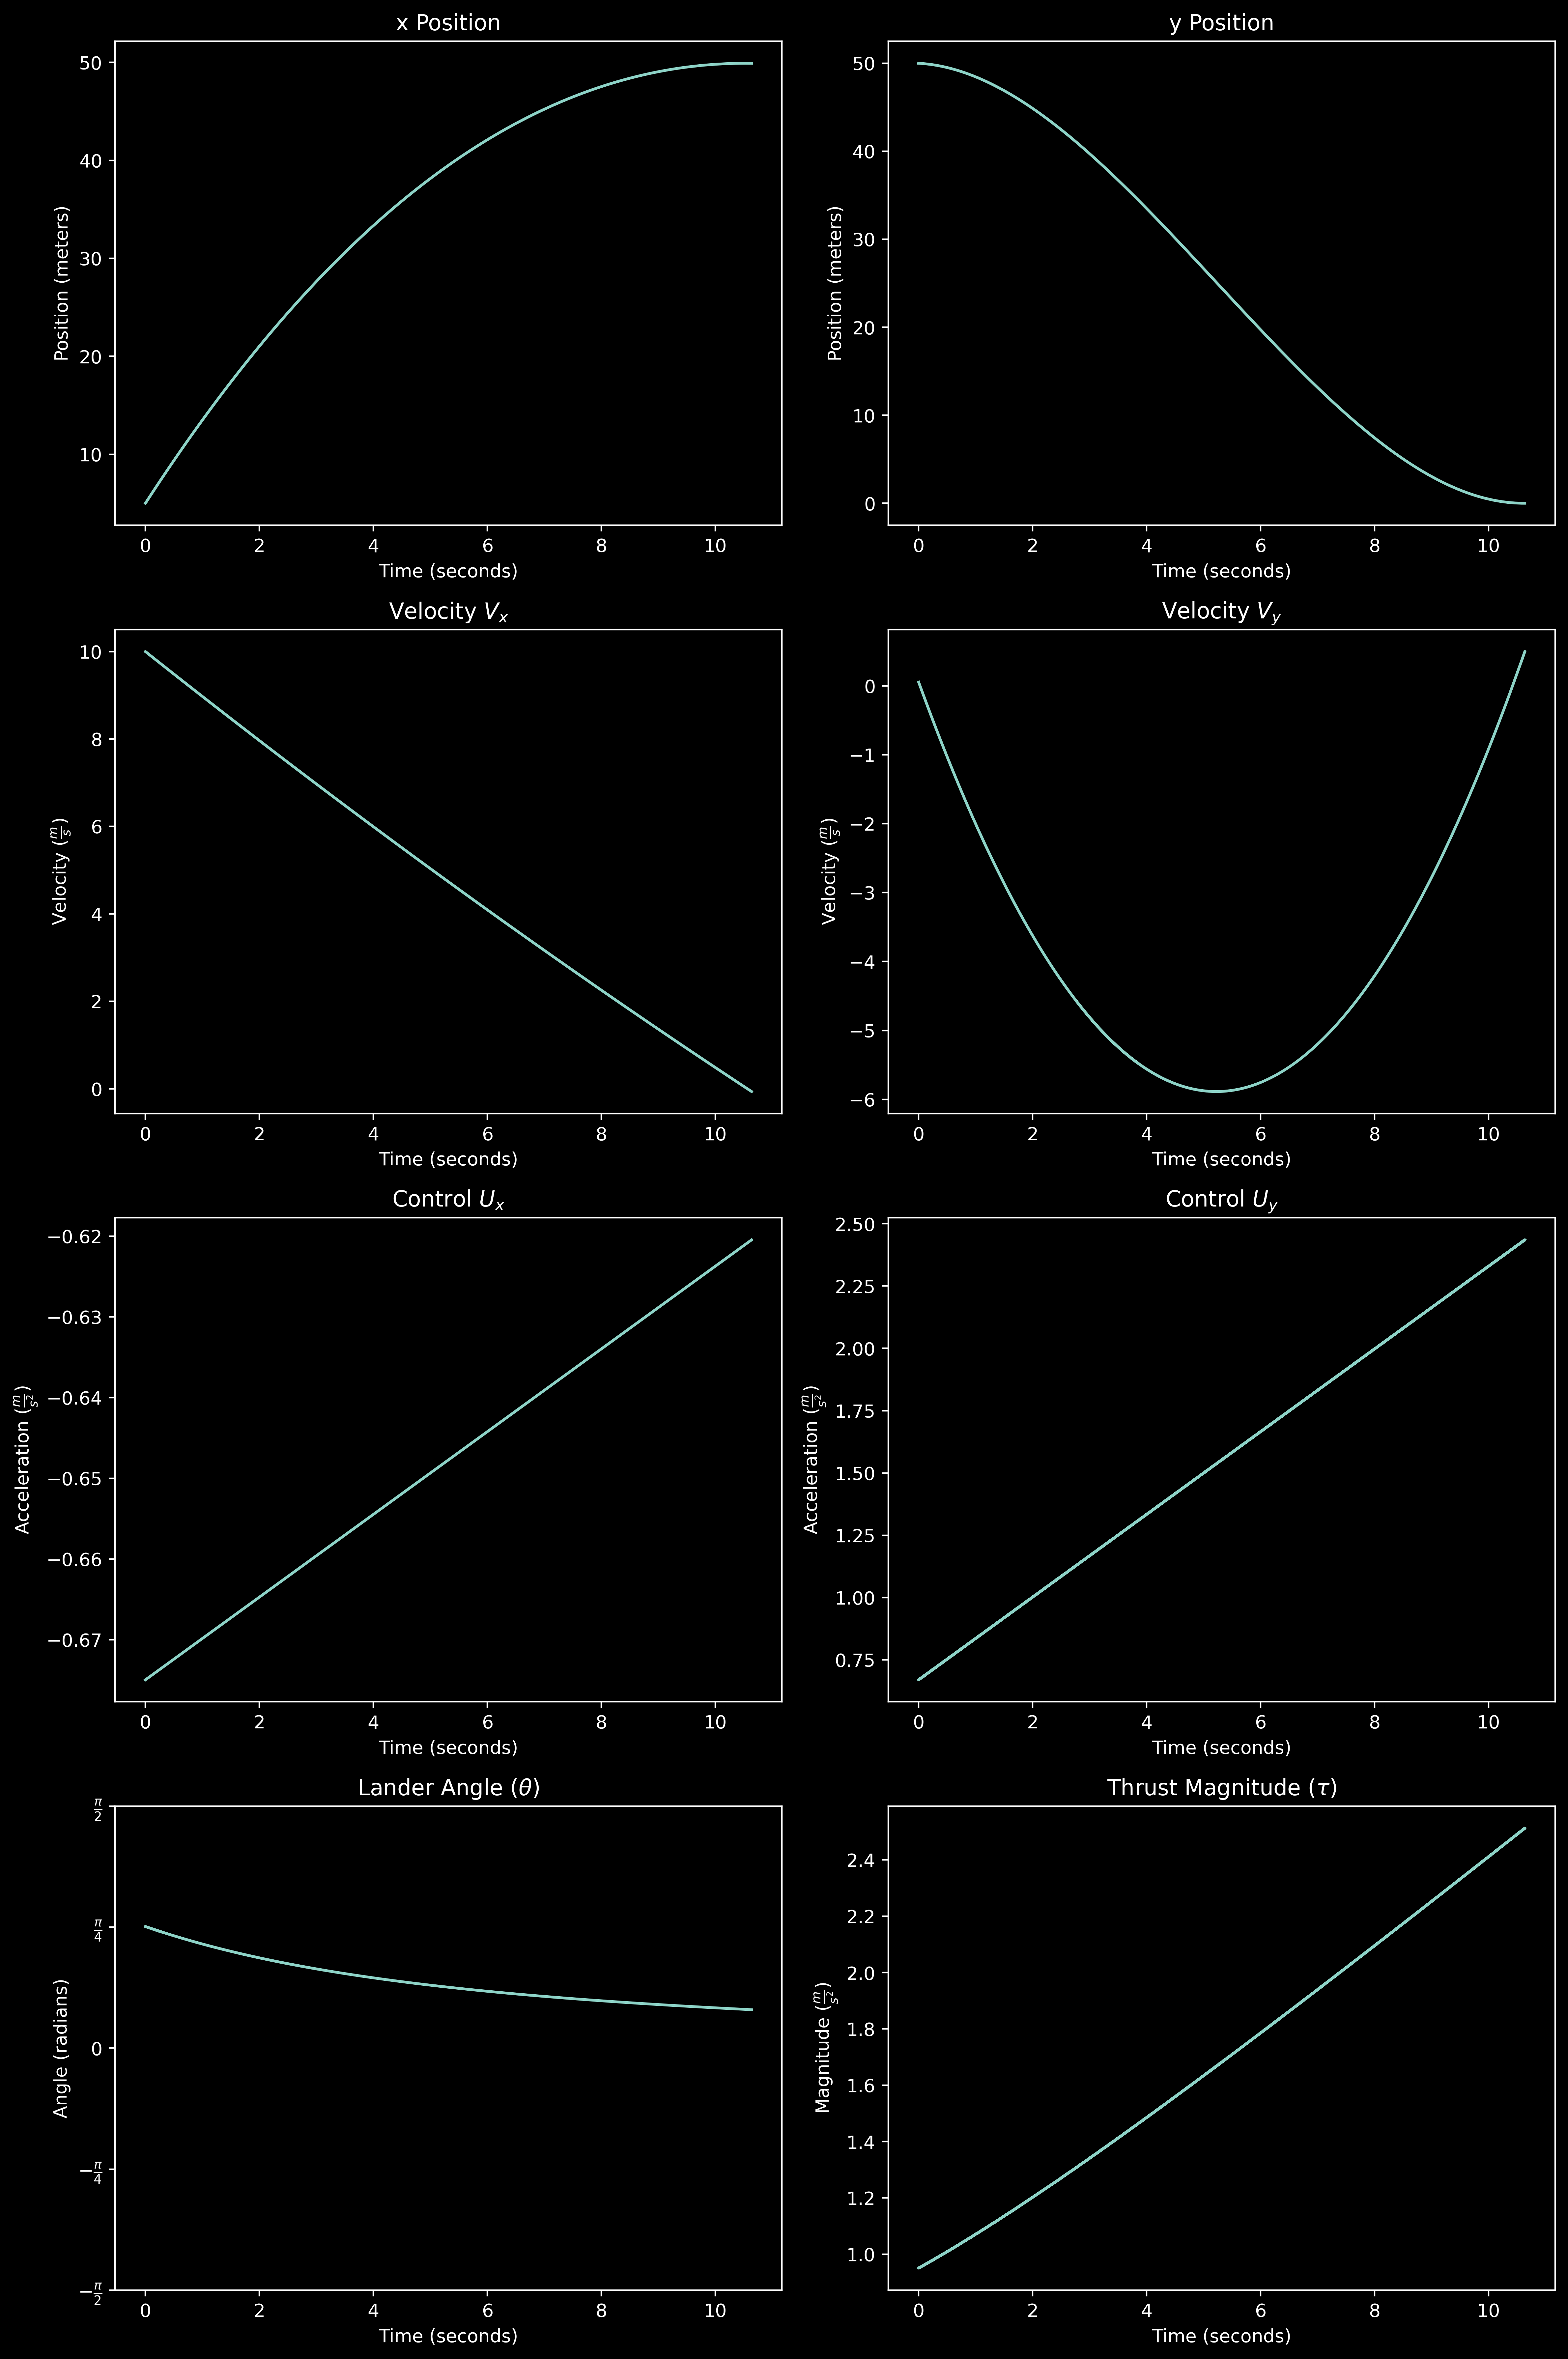
\includegraphics[width=1\linewidth,trim={0 0cm 0cm 0cm},clip]{full_output.png}
        % \end{cen ter}
        

        \vspace{2cm}




            % \columnbreak

    \FancySubtitle[4mm][1cm]{Early Results \& \\[1ex]Analysis}
        
We have found that our modeling produces numerical solutions that match both our intuition and the actual gameplay of "Lunar Lander". Through analysis of the trajectory of the lander and velocity, we found that the vertical position steadily decreases to zero (the lunar surface). The horizontal position increased quickly at first because of the initial velocity and then slowed down as time progressed. The velocity steadily decreased towards zero to prevent the lander from tipping over when it lands. The vertical velocity starts at zero, decreases to allow the rocket to move downwards, and then goes back up to zero for a softer landing.
The plots below show the optimal trajectory and controls and depict how the lander can rotate as it approaches the ground.
    


   \FancySubtitle[4mm][1cm]{Conclusions and next\\[1ex]steps}


In the future, we will consider a non-uniform lunar surface, as shown in the first image below, where the lander is rewarded for landing in flat areas and certain areas with point bonuses. Also, to mimic the actual gameplay, we also want the spacecraft to land nearly perpendicular to the moon's surface, so we plan to implement an inequality constraint on the lander's final angle. It would be interesting to adjust our functional to account for obstacles, both on the ground and in the air, that the lander must dodge. Some of these obstacles may be asteroids or steep landscapes that are impossible for the craft to land on.

    % \bibliographystyle{amsalpha}
    % \bibliography{poster_references}

%     \renewcommand{\refname}{\vspace*{-0.5cm}}  % Move title up
% {\small
% \setlength{\itemsep}{-1ex}
% \setlength{\parskip}{0pt}
% \setlength{\parsep}{0pt}
% \bibliographystyle{plain}  % Most compact standard style
% \bibliography{poster_references}}

% \noindent\textbf{\color{white}References}\vspace{-2mm}  % Add heading and reduce space below
{\small
\setlength{\itemsep}{-1ex}
\setlength{\parskip}{0pt}
\setlength{\parsep}{0pt}
\bibliographystyle{plainurl}  % Most compact standard style
\bibliography{poster_references}}
\end{multicols*}
\end{minipage}


\vspace{1in}


\begin{minipage}{\linewidth + 2\fboxsep}
\begin{multicols*}{3}
\begin{center}
\begin{tcolorbox}[width=0.85\linewidth]
    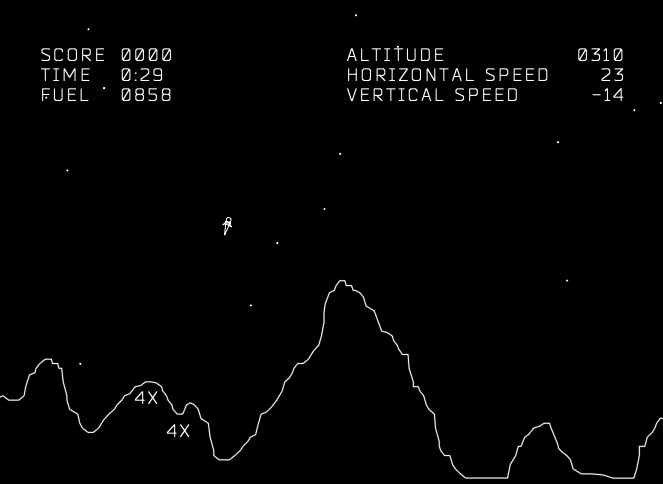
\includegraphics[width=\linewidth,trim={0 .2cm 0 1.3cm},clip]{lunar_lander_gameplay.png}
\end{tcolorbox}
\end{center}
\Large 
Image from~\cite{LunarLander}.

\columnbreak

% If you save figures from matplotlib with a 1.5 aspect ratio (so figure.figsize = [9, 6] for example),
% then you will not need to crop them at all once you put them in here

\begin{center}
\begin{tcolorbox}[width=0.67\linewidth]
    \includegraphics[width=\linewidth,trim={0 0 0 0},clip]{thing_v2.jpg}
\end{tcolorbox}
\end{center}


\columnbreak

\begin{center}
\begin{tcolorbox}[width=0.85\linewidth]
    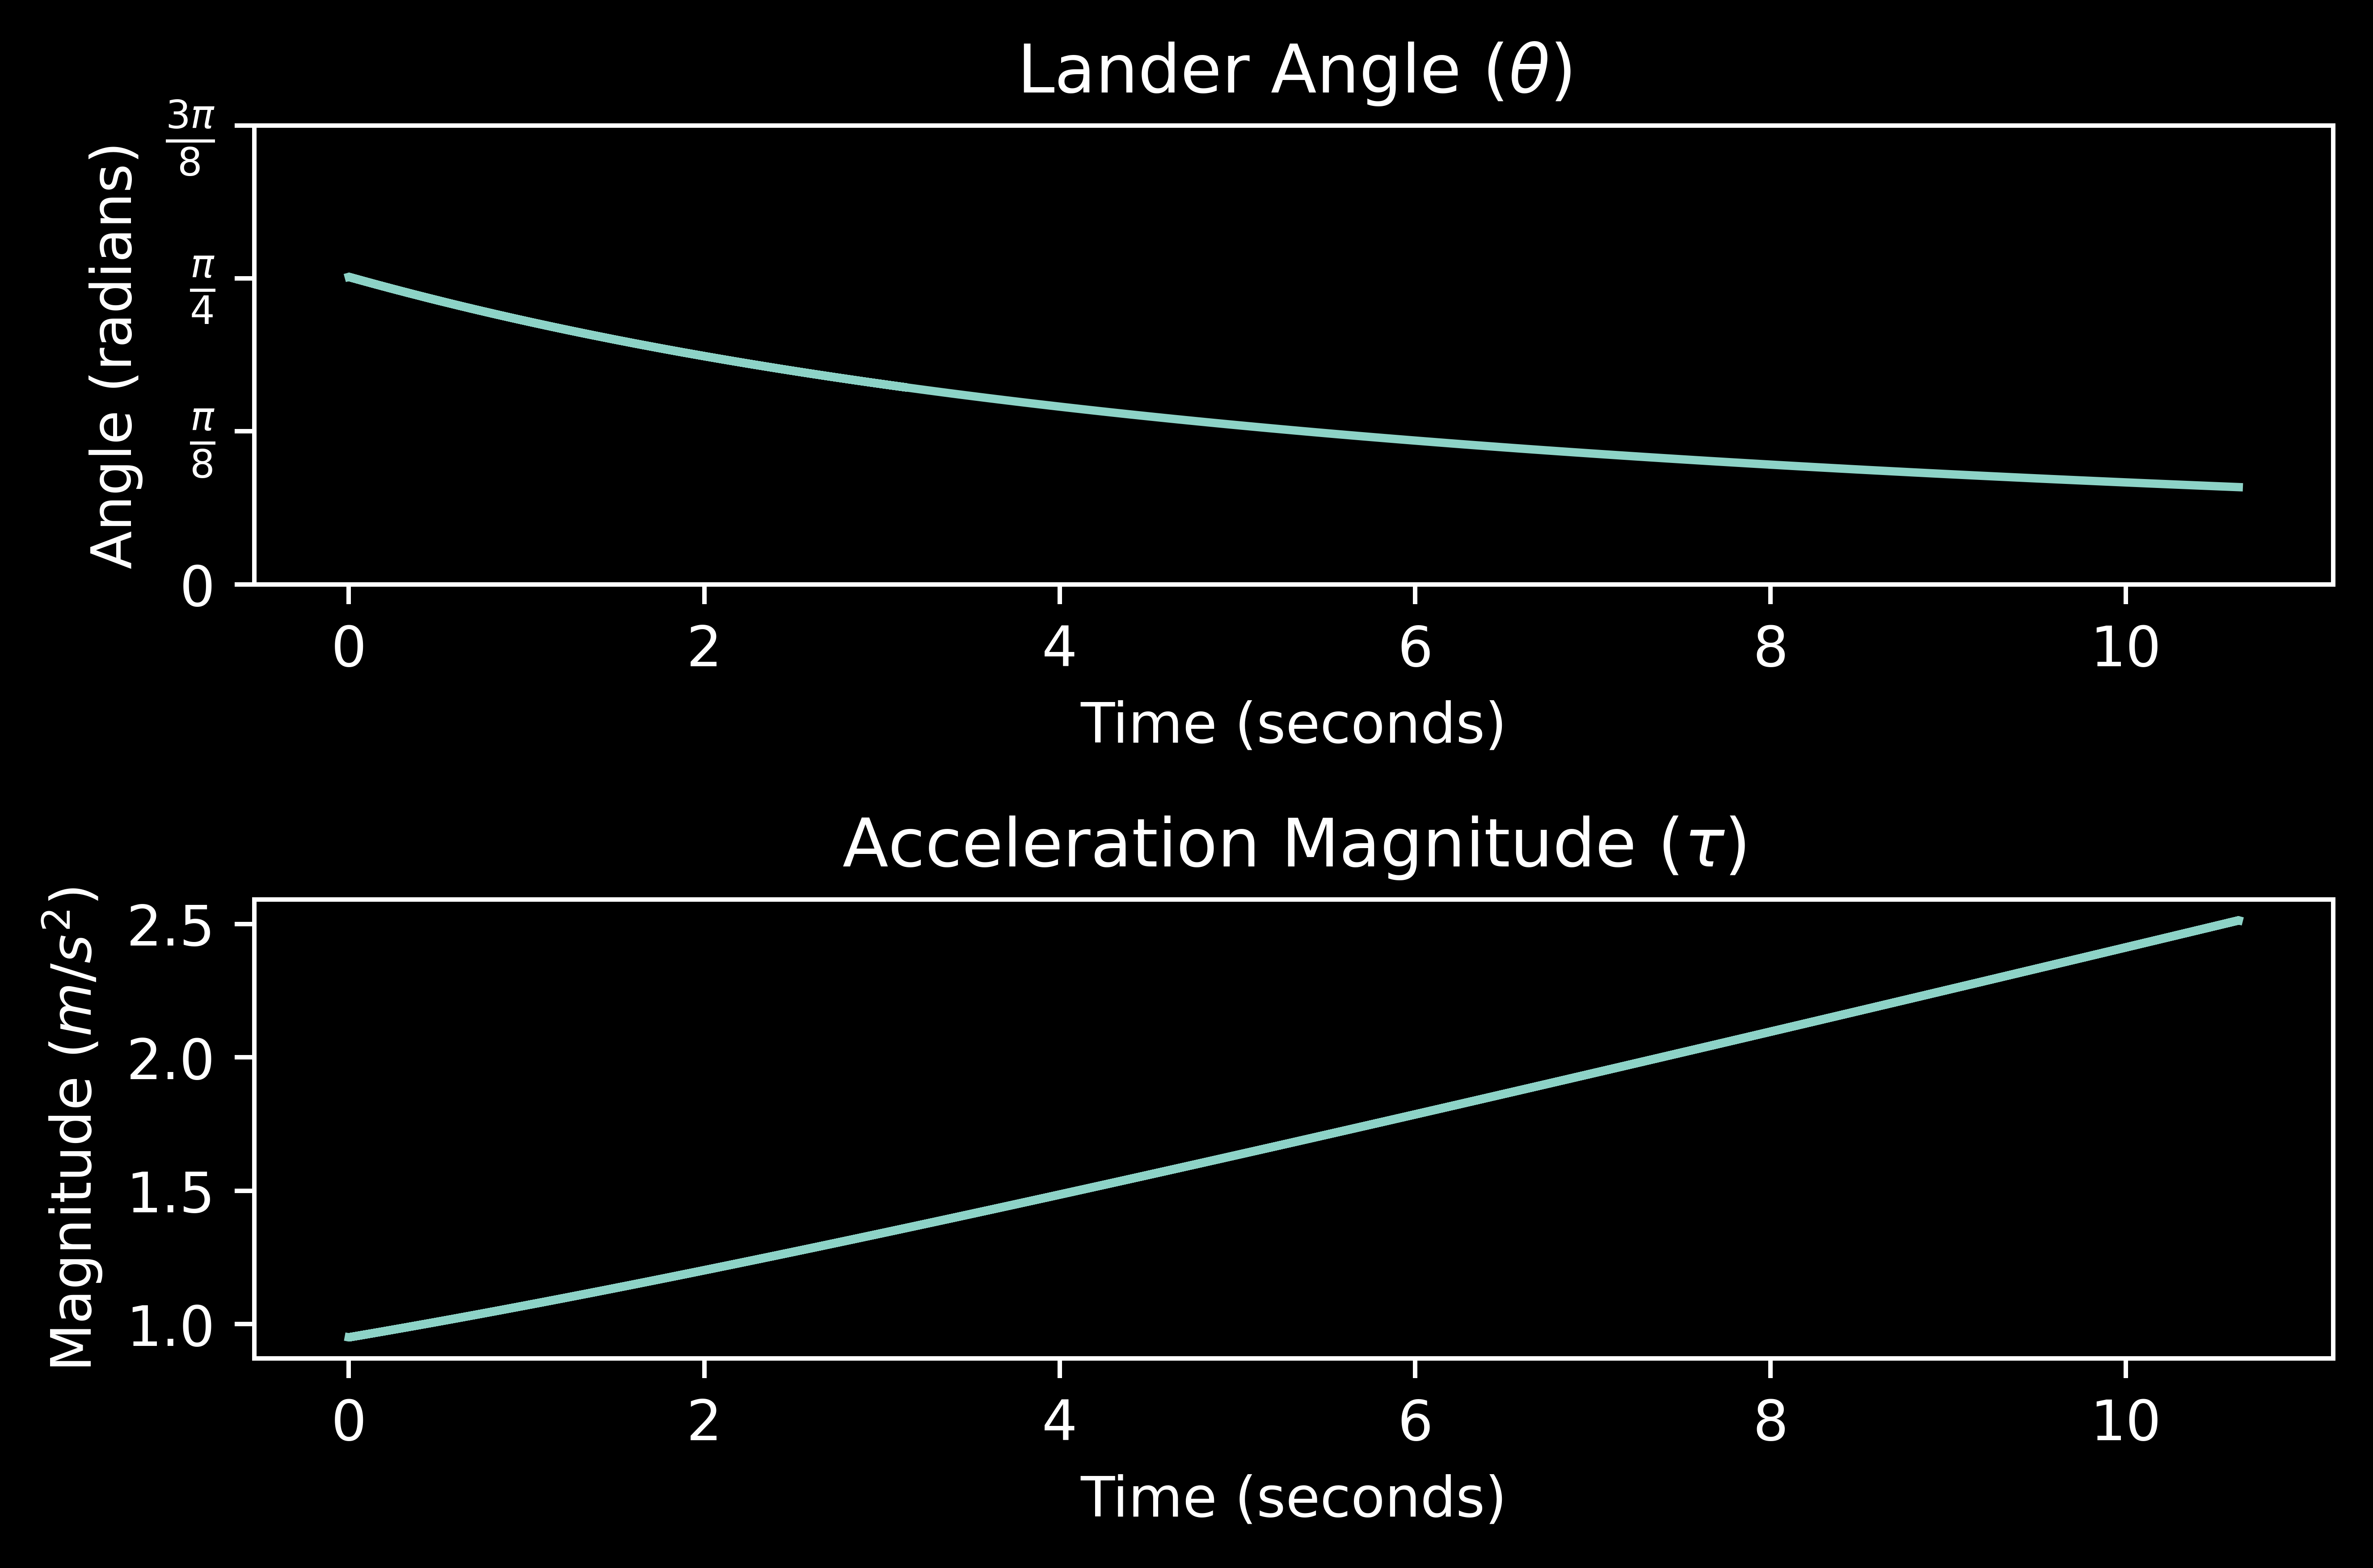
\includegraphics[width=\linewidth,trim={0 0.6cm 0 0.6cm},clip]{control_output.pdf}
\end{tcolorbox}
% \FancyFigure{control_output.pdf}{The rotation angle and acceleration magnitude computed from $u_x$ and $u_y$} \label{fig:controls}
\end{center}

\end{multicols*}
% Put new 

\end{minipage}

\nocite{unsplash}
%Using nocite allows a reference to appear in the reference list without a citation appearing in the poster.
\footnotesize

\end{document}